
% Quine quotation.

This chapter will describe an implementation of \algo which uses
Nested Data Parallelism in Haskell (by \cite{Harness2008}).
First, a a few predefined functions will be presented to
increase their the understanding of their operational behavior.
Then the implementation will be presented and it's complexities will
calculated.

\section{Utilities}

  \subsection{Scanl}
    Parallel prefix sum has well studied efficient implementaitons. One of them
    is the following:
    \begin{lstlisting}   
scanlP f z xs =
joinD
. mapD (\(as,a) -> mapS (f a) as)
. propagateD f z
. mapD (scanlS f z)
. splitD
$ xs
    \end{lstlisting}
    This implementatin is designed to reduce communication
    and therefore increase efficiency. It works in three steps.
    First, each PU computes its local prefix sum (line 5).
    Second, the total sum of each of the PUs is propagated
    - adding up subsequent values (line 4).
    Third, the updated sum is used to increase the values of the local chunks (line 39).
    This approach is visualised in \ref{figure:scanlPsteps}
    
    \begin{figure}[h!]
        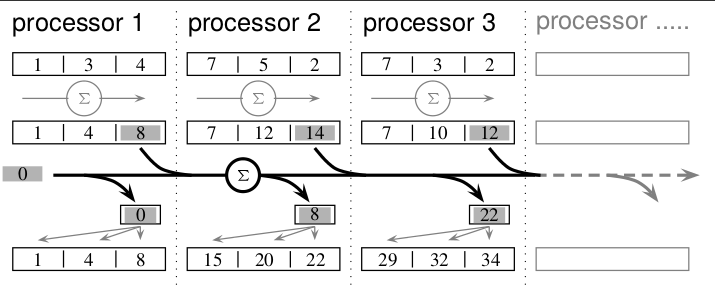
\includegraphics[width=\linewidth]{scanlP-three-steps.png}
        \caption{Parallel prefix sum in three steps (Figure from \cite{DistTypes1999}) }
        \label{figure:scanlPsteps}
    \end{figure}
    The propagation is the bottle neck in terms of dpeth and parallel complexity.
    But since the progapation itself is structurally isomorphic to prefix summing itself,
    we can use a different efficient scheme for propagation for the local values distributed on the PUs.
    This propagation can in fact be done in a time logarithmic to the number of PUs!
    It an be derived from \cite{Scanl1980}. For our purposes, it is sufficient to know the following complexities for scanlP:
    $\W(n) \in O(n)$ and $\D(n) \in O(\log n)$.

  \subsection{GroupP}
    \c{groupP} is a frequently used function in functional programming.
    It's type is \type{[:a:] -> [:[:a:]:]} and given an array it returns an array of arrays,
    where each subarray contains equal consecutive
    elements of the source array. For example
    \c{groupP [4,2,2,2,2,3,3,1]} becomes \c{[[4],[2,2,2,2],[3,3],[1]]}.
    In NDP, the latter is represented by
    \begin{lstlisting}
AArr {
data = [# 4,2,2,2,3,3,1 #],
segd = ATup2 {
  as = [# 0,1,5,7 #]
  bs = [# 1,4,2,1 #]
}
}
    \end{lstlisting}
    An efficient parallel implementation of \c{groupP}
    relies on the following key insight - the \c{data} field in the nested array
    is the source array itself! To implement \c{groupP} we only
    need to efficiently calculate the segment descriptor field. This is
    possible in depth logarithmic to the size of the input array!
    
    \begin{figure}[h!]
        \begin{center}
        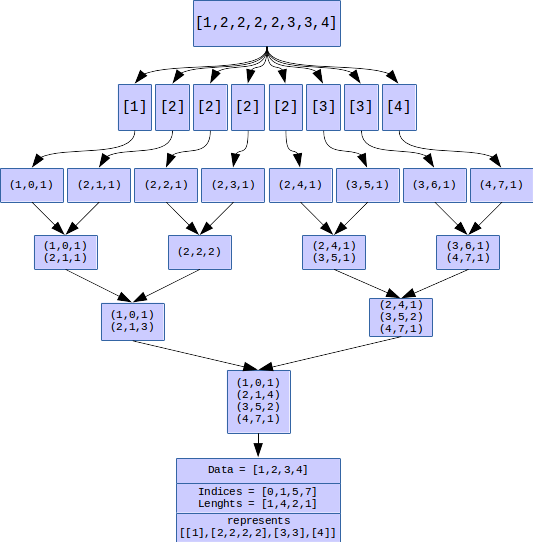
\includegraphics[width=\linewidth]{groupP.png}
        \caption{An example calculation of groupP. Each box is a PU.}
        \label{figure:groupP}
        \end{center}
    \end{figure}
    
    As visualised in the figure \ref{figure:groupP}
    we can do that by spliting all elements onto all PUs first.
    Then each PU creates a local chunk of a linked list of
    \c{(Value,StartIdx,Count)}-Triplets to record it singleton.
    After that, each level of recursion merges two PUs by
    merging the last triplet of the left list with the first triplet
    of the right list. If both triplets correspond to the same value,
    then a new triplet with the total count and the left index is used.
    If both are unequal, then they are left unchanged. The implementation
    of \c{groupP} uses a subfunction \c{segdSplitMerge} to implement the
    splitting and merging. This function will be exposed lateron in
    the vectorization of \ndpn.
    Further analysis reveals the complexities $\W(n) \in O(n)$ and $\D(n) \in O(\log n)$.
    All in all, \c{groupP} is an operation which can very well exploit the flat representation of nested arrays.
    % TODO: and to appendix and refer ot it?
    
  \subsection{SortP}
    General parallel sorting can be as simple as a parallel
    implementation of merge-sort where the recursive calls are executed
    in parallel. \c{sortP} of type \type{[:a:] -> [:a:]} implements this,
    and optimal complexities of $\W(n) \in O(n \log n)$
    and $\D(n) \in O(\log n)$.
    \footnote{There exists other sorting mechanism
    like \emph{Batcher's Bitonic Sort} with $O(n \log^2 n)$ work and $O(\log^2 n)$
    depth. I did not use its implementation as it is sophisticated and
    the workload of its vectorization would have been enourmous (on top of the work I already had).
    Retrospectively, I didn't end up opening and inlining the \c{sortP} in \ndpn - but that
    was not clear beforehand.
    }
    % TODO: cite. Parallel mergesort with work and depth.
    % TODO: cite batchers bitonic sort

  \subsection{Histogram calculation}
    Conventional functional programming very often enables us to write
    consise and correct implementations of functionality on ordered
    data structures (like lists and arrays). For example - consider the problem of run length encoding.
    Given a (possibly long) array, the goal is to create a sparse array
    that compresses elements by encoding consecutive equal elements
    with a tuple of the element and its number of occurrences.
    E.g. it transformes \c{[4,2,2,2,2,3,3,1]} to \c{[(4,1),(2,4),(3,2),(1,1)]}.
    An implementation is straightforward in functional programming.
    \begin{lstlisting}
runLengthEncode :: [:a:] -> [:(a,Int):]
runLengthEncode = mapP (\xs -> (headP xs, lengthP xs)) . groupP
    \end{lstlisting}
    This function uses \c{groupP} to first create subarrays of
    equal consecutive elements. Then - all it needs to do - is to
    transform subarrays like \c{[2,2,2,2]} to tuples like \c{(2,4)}.
    That is the second step of run length encoding.
    
    But how is this going to be helpful for creating a histogram?
    
    We could try applying run length encoding on the images pixels. However,
    for that we need to take care of two subtilities. First, the image
    has the type \type{[:[:a:]:]}. So we need to first flatten
    it with \c{concatP}\footnote{It's type is \type{[:[:a:]:] -> [:a:]}}
    before we can continue. Once we have the flatten image,
    we, secondly, have the problem that the pixels are unordered - 
    and that run length encoding wouldn't create any useful result 
    because we need to count together all occurrences of the same
    gray tone. A simple solution to that is sorting the image beforhand (using \c{sortP}).
    Afterwards, we finally have a histogram of the image.
    We end up with an array of type \type{[:(Int,Int):]} where each element
    describes a gray tone (first integer in tuple) and its number of
    occurrences (second integer in tuple).
    Using this approach, we have a parallel implementation histogram calculation,
    without having had to put much thought. This is in constrast
    to our implementaiton in \man.
    
\section{Implementation}
  After a small introduction of a few utilities and a description of how
  parallel histogram calculcation can be implemented - we are now ready to
  take a look at the implemetation. The code
  implements \algo using Nested Data Parallelism in Haskell and
  might look like this:
  \begin{lstlisting}
type Image = [:[:Int:]:]
type Hist a = [:a:]

hbalance :: Image -> Image
hbalance img =
  let h = hist img
      a = accu h
      a0 = headP a
      agmax = lastP a
      n = normalize a0 agmax a
      s = scale gmax n
      img' = apply s img
  in  img'

hist :: Image -> Hist Int
hist = sparseToDenseP (gmax+1) 0
        . mapP (\g -> (headP g,lengthP g))
        . groupP
        . sortP
        . concatP

accu :: Hist Int -> Hist Int
accu = scanlP (+) 0

normalize :: Int -> Int -> Hist Int -> Hist Double
normalize a0' agmax' as =
  let a0 = fromIntegral a0'
      agmax = fromIntegral agmax'
      divisor = agmax - a0
  in  [: (fromIntegral freq' - a0) / divisor | freq' <- as :]

scale :: Int -> Hist Double -> Hist Int
scale gmax as = [: floor (a * fromIntegral gmax) |  a <- as :]

apply :: Hist Int -> Image -> Image
apply as img = mapP (mapP (as !:)) img
  \end{lstlisting}
  The first two lines describe the data structure we are using to encode an image - 
  manely nested data-parallel arrays.
  As decribed in the basics chapter - in NDP
  nested arrays are converted to flat data and a segment decsriptor
  during vectorization - so there is no overhead in using nesting.
  Our implementation - like in the pseudocode and in \seq - 
  is split up in histogram calculation (lines 20 - 16)
  \footnote{The lines are intentionally counted backwards. This is due to the right-assosiativity of function composition - e.g. \c{h . g . f} applies f first, then g and finally h.}
  ,histogram accumulcation (line 23), normalisation (line 26 - 30),
  scaling (line 33) and the final gray tone mapping (line 36).
  The implementation operationally only differs in the histogram calculation from \seq.
  (Aside from the fact, that \seq uses a binary-search-tree instead of an array
  for the gray tones.)
  Histogram calculation is implemented based on the approach explained in the
  previous section. We first, flatten the array, then sort it and afterwards
  use run length encoding.
  
  At the end, however, we have to call a function
  named \c{sparseToDenseP size z}\footnote{Its type is  \type{Int -> a -> PA (Int,a) -> PA a}}
  to convert the sparse array \type{[:(Int,Int):]} to its corresponding
  dense array \type{[:Int:]}. The dense array has size \c{size} and
  inserts \c{z} for elements not specified in the sparse array
  \footnote{E.g. \c{ sparseToDenseP 8 0 [: (1,5),(2,4),(6,7) :] => [: 0,5,4,0,0,0,7,0 :]}}
  .
  Using this approach, \c{hist} can finally create an array where
  the element at the index \c{i} is the number of occurrences
  of the gray tone \c{i} in the original image. This is
  a simpler format for the same histogram.\footnote{Keeping sparse arrays for the representation of the histogram is a viable option yielding possibly different (maybe better?) complexities.}
  
  At last, we shall consider the function \c{apply}. It uses a nested
  application of parallel functions and be subject to flattening in \ndpv.
  
\section{Complexities}
  
  
  % TODO: Genau erläuteren und präzisieren wie Work&Depth mit der Anzahl der Prozessoren in den distributed Types zusammenhängen.
  %    Die tatsächliche Parallelität steck in der Anzahl der PUs (Processing Units) und den verteilten Algorithmen
  %    zwischen den einzelnen PUs. Damit wird sumD und propagateD auf D(log n) gedrückt.
      
  % Ignoriert!! Twofold interpretation: divL = <built-in parallel divL> OR < mapD divS> with distributed types and extended library optimization
  % immer die zweite variante - weil sonst das andere Pman program nicht ginge.
    
  
